\documentclass[10pt,aspectratio=169,serif]{beamer}

\usepackage[fontset=none, scheme=plain]{ctex}
\IfFontExistsTF{Songti SC}{%
	\setCJKmainfont{Songti SC}[AutoFakeSlant=0.2]%
	\setCJKsansfont{Songti SC}[AutoFakeSlant=0.2]%
}{%
	\setCJKmainfont{FandolSong-Regular}[Extension=.otf,BoldFont=FandolSong-Bold,AutoFakeSlant=0.2]%
	\setCJKsansfont{FandolSong-Regular}[Extension=.otf,BoldFont=FandolSong-Bold]%
}
\usepackage{amsmath,amssymb,graphicx,tikz,booktabs,multicol,calligra}
\usepackage{pgfplots}
\pgfplotsset{compat=1.18}
\usepackage{tcolorbox}
\tcbuselibrary{skins}
\usepackage{XyygU}
\usepackage{caption}
\captionsetup[figure]{name=图,labelsep=period}

\usetikzlibrary{arrows.meta,positioning,calc}

% 公式间距
\setlength{\abovedisplayskip}{0pt plus 2pt minus 2pt}
\setlength{\belowdisplayskip}{0pt plus 2pt minus 2pt}

\title[集合的基本运算练习]{1.3 集合的基本运算（练习）}
\subtitle{交集、并集与补集}
\author{}
\institute{}
\date{2026-10-16}

\begin{document}

\begin{frame}
  \titlepage
\end{frame}

% ========== 第一部分：交集与并集（教材P12练习） ==========
\begin{frame}[t]{第一部分：交集与并集（教材第12页练习）}
本部分为教材第12页"练习"，共4题，围绕\alert{交集}与\alert{并集}的概念。

\vspace{1em}
\textbf{核心定义：}
\begin{tcolorbox}[colback=blue!5,colframe=blue,title=\textbf{交集与并集}]
\textbf{交集：} $A \cap B = \{x \mid x \in A \text{ 且 } x \in B\}$\\[0.3em]
\textbf{并集：} $A \cup B = \{x \mid x \in A \text{ 或 } x \in B\}$
\end{tcolorbox}
\end{frame}

% ===== 练习1-1 =====
\begin{frame}[t]{练习1：列举法求交集并集}
\textbf{1.} 设 $A = \{3, 5, 6, 8\}$，$B = \{4, 5, 7, 8\}$，求 $A \cap B$，$A \cup B$。
\end{frame}

\begin{frame}[t]{练习1 解答}
\begin{tcolorbox}[colback=orange!10,colframe=orange,title=\textbf{解}]
\textbf{找公共元素：} $A$ 与 $B$ 共有的元素为 $5, 8$，故
\[
A \cap B = \{5, 8\}.
\]
\textbf{合并所有元素：} 将 $A, B$ 元素合并（重复元素只写一次），故
\[
A \cup B = \{3, 4, 5, 6, 7, 8\}.
\]
\vspace{0.5em}
\small（注意：$5, 8$ 在两个集合中都出现，并集中只列一次）
\end{tcolorbox}
\end{frame}

% ===== 练习1-2 =====
\begin{frame}[t]{练习2：方程解集的交并}
\textbf{2.} 设 $A = \{x \mid x^2 - 4x - 5 = 0\}$，$B = \{x \mid x^2 = 1\}$，求 $A \cup B$，$A \cap B$。
\end{frame}

\begin{frame}[t]{练习2 解答}
\begin{tcolorbox}[colback=orange!10,colframe=orange,title=\textbf{解}]
\textbf{先化简集合：}\\
解方程 $x^2 - 4x - 5 = 0$，即 $(x-5)(x+1)=0$，得 $x = 5$ 或 $x = -1$，故
\[
A = \{-1, 5\}.
\]
解方程 $x^2 = 1$，得 $x = \pm 1$，故
\[
B = \{-1, 1\}.
\]
\textbf{求交并：}
\[
A \cap B = \{-1\},\qquad A \cup B = \{-1, 1, 5\}.
\]
\end{tcolorbox}
\end{frame}

% ===== 练习1-3 =====
\begin{frame}[t]{练习3：描述法求交并}
\textbf{3.} 设 $A = \{x \mid x \text{ 是等腰三角形}\}$，$B = \{x \mid x \text{ 是直角三角形}\}$，求 $A \cap B$，$A \cup B$。
\end{frame}

\begin{frame}[t]{练习3 解答}
\begin{tcolorbox}[colback=orange!10,colframe=orange,title=\textbf{解}]
\textbf{交集：} 同时满足"等腰"和"直角"两个条件，即等腰直角三角形：
\[
A \cap B = \{x \mid x \text{ 是等腰直角三角形}\}.
\]
\textbf{并集：} 满足"等腰"或"直角"至少一个条件：
\[
A \cup B = \{x \mid x \text{ 是等腰三角形或直角三角形}\}.
\]
\vspace{0.5em}
\small（注意："等腰三角形或直角三角形"包括等腰非直角、直角非等腰、等腰直角三类）
\end{tcolorbox}
\end{frame}

% ===== 练习1-4 =====
\begin{frame}[t]{练习4：实际情境中的并集}
\textbf{4.} 设 $A = \{x \mid x \text{ 是幸福农场的汽车}\}$，$B = \{x \mid x \text{ 是幸福农场的货车}\}$，求 $A \cup B$。
\end{frame}

\begin{frame}[t]{练习4 解答}
\begin{tcolorbox}[colback=orange!10,colframe=orange,title=\textbf{解}]
货车属于汽车的一种（汽车是机动车的统称，包括客车、货车等），因此
\[
B \subseteq A.
\]
由 $B \subseteq A$，得
\[
A \cup B = A = \{x \mid x \text{ 是幸福农场的汽车}\}.
\]
\vspace{0.5em}
\small（若货车全部属于农场的汽车范畴，则并集就是农场的全部汽车）
\end{tcolorbox}
\end{frame}

% ========== 第二部分：补集（教材P13练习） ==========
\begin{frame}[t]{第二部分：补集（教材第13页练习）}
本部分为教材第13页"练习"，共3题，围绕\alert{补集}的概念。

\vspace{1em}
\begin{tcolorbox}[colback=blue!5,colframe=blue,title=\textbf{全集与补集}]
\textbf{全集：} 含研究问题中所有元素的集合，记作 $U$。\\[0.3em]
\textbf{补集：} $\complement_U A = \{x \mid x \in U \text{ 且 } x \notin A\}$
\end{tcolorbox}
\end{frame}

% ===== 练习2-1 =====
\begin{frame}[t]{练习5：补集与交并混合}
\textbf{1.}（补集练习第1题）已知 $U = \{1, 2, 3, 4, 5, 6, 7\}$，$A = \{2, 4, 5\}$，$B = \{1, 3, 5, 7\}$，求 $A \cap (\complement_U B)$，$(\complement_U A) \cap (\complement_U B)$。
\end{frame}

\begin{frame}[t]{练习5 解答}
\begin{tcolorbox}[colback=orange!10,colframe=orange,title=\textbf{解}]
\textbf{先求补集：}
\[
\complement_U A = \{1, 3, 6, 7\},\qquad \complement_U B = \{2, 4, 6\}.
\]
\textbf{第一问：}
\[
A \cap (\complement_U B) = \{2, 4, 5\} \cap \{2, 4, 6\} = \{2, 4\}.
\]
\textbf{第二问：}
\[
(\complement_U A) \cap (\complement_U B) = \{1, 3, 6, 7\} \cap \{2, 4, 6\} = \{6\}.
\]
\vspace{0.5em}
\small（由德摩根律，$(\complement_U A)\cap(\complement_U B)=\complement_U(A\cup B)=\{6\}$）
\end{tcolorbox}
\end{frame}

% ===== 练习2-2 =====
\begin{frame}[t]{练习6：图形分类中的补集}
\textbf{2.}（补集练习第2题）设 $S = \{x \mid x \text{ 是平行四边形或梯形}\}$，$A = \{x \mid x \text{ 是平行四边形}\}$，$B = \{x \mid x \text{ 是菱形}\}$，$C = \{x \mid x \text{ 是矩形}\}$，求 $B \cap C$，$\complement_A B$，$\complement_S A$。
\end{frame}

\begin{frame}[t]{练习6 解答}
\begin{tcolorbox}[colback=orange!10,colframe=orange,title=\textbf{解}]
\textbf{(1) $B \cap C$：} 既是菱形又是矩形的四边形是正方形，故
\[
B \cap C = \{x \mid x \text{ 是正方形}\}.
\]
\textbf{(2) $\complement_A B$：} 在平行四边形 $A$ 中去掉菱形 $B$，即邻边不都相等的平行四边形：
\[
\complement_A B = \{x \mid x \text{ 是邻边不都相等的平行四边形}\}.
\]
\textbf{(3) $\complement_S A$：} 在 $S$ 中去掉平行四边形 $A$，剩下梯形：
\[
\complement_S A = \{x \mid x \text{ 是梯形}\}.
\]
\end{tcolorbox}
\end{frame}

% ===== 练习2-3 =====
\begin{frame}[t]{练习7：Venn图表示补集运算}
\textbf{3.}（补集练习第3题）图中 $U$ 是全集，$A$，$B$ 是 $U$ 的两个子集，用阴影表示：\\
(1) $(\complement_U A) \cap (\complement_U B)$；\qquad (2) $(\complement_U A) \cup (\complement_U B)$。

\vspace{1em}
\begin{center}
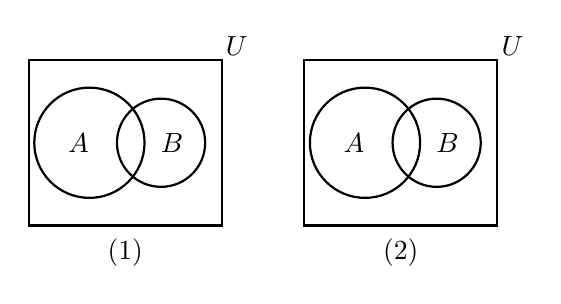
\begin{tikzpicture}[scale=0.7]
% 左图
\draw[thick] (0,0) rectangle (3.5,3);
\node[above right] at (3.4,2.9) {$U$};
\draw[thick] (1.1,1.5) circle (1);
\draw[thick] (2.4,1.5) circle (0.8);
\node at (0.9,1.5) {$A$};
\node at (2.6,1.5) {$B$};
\node at (1.75,-0.5) {(1)};
% 右图
\begin{scope}[xshift=5cm]
\draw[thick] (0,0) rectangle (3.5,3);
\node[above right] at (3.4,2.9) {$U$};
\draw[thick] (1.1,1.5) circle (1);
\draw[thick] (2.4,1.5) circle (0.8);
\node at (0.9,1.5) {$A$};
\node at (2.6,1.5) {$B$};
\node at (1.75,-0.5) {(2)};
\end{scope}
\end{tikzpicture}
\end{center}
\end{frame}

\begin{frame}[t]{练习7 解答}
\begin{tcolorbox}[colback=orange!10,colframe=orange,title=\textbf{解（德摩根律）}]
由\alert{德摩根律}：
\[
(\complement_U A)\cap(\complement_U B)=\complement_U(A\cup B),\qquad
(\complement_U A)\cup(\complement_U B)=\complement_U(A\cap B).
\]
\textbf{(1)} $(\complement_U A)\cap(\complement_U B)$：$U$ 中去掉 $A\cup B$ 后的部分，即矩形内除去两圆合并区域之外的部分。\\[0.5em]
\textbf{(2)} $(\complement_U A)\cup(\complement_U B)$：$U$ 中去掉 $A\cap B$（两圆重叠部分）后的部分，即除两圆相交区域外全部涂阴影。
\end{tcolorbox}
\end{frame}

\begin{frame}[t]{练习7 配图：阴影结果}
\begin{center}
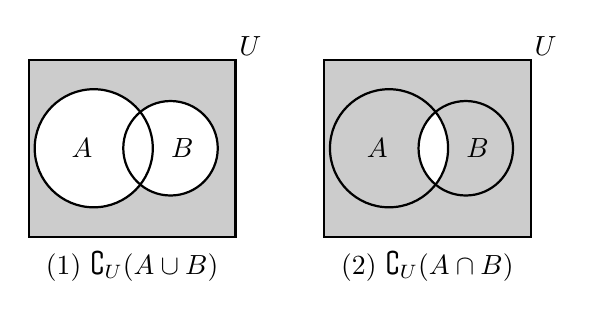
\begin{tikzpicture}[scale=0.75]
% 左图：(1) = 矩形去掉 A∪B
\fill[gray!40] (0,0) rectangle (3.5,3);
\fill[white] (1.1,1.5) circle (1);
\fill[white] (2.4,1.5) circle (0.8);
\draw[thick] (0,0) rectangle (3.5,3);
\node[above right] at (3.4,2.9) {$U$};
\draw[thick] (1.1,1.5) circle (1);
\draw[thick] (2.4,1.5) circle (0.8);
\node at (0.9,1.5) {$A$};
\node at (2.6,1.5) {$B$};
\node at (1.75,-0.5) {(1) $\complement_U(A\cup B)$};

% 右图：(2) = 去掉 A∩B
\begin{scope}[xshift=5cm]
\fill[gray!40] (0,0) rectangle (3.5,3);
% 挖掉A圆和B圆，只保留交集白色
\begin{scope}
\fill[white] (1.1,1.5) circle (1);
\fill[white] (2.4,1.5) circle (0.8);
\end{scope}
% 交集区域涂灰
\fill[gray!40] (1.1,1.5) circle (1);
\fill[gray!40] (2.4,1.5) circle (0.8);
% 重新画交集为白色
\begin{scope}
\clip (1.1,1.5) circle (1);
\fill[white] (2.4,1.5) circle (0.8);
\end{scope}
\draw[thick] (0,0) rectangle (3.5,3);
\node[above right] at (3.4,2.9) {$U$};
\draw[thick] (1.1,1.5) circle (1);
\draw[thick] (2.4,1.5) circle (0.8);
\node at (0.9,1.5) {$A$};
\node at (2.6,1.5) {$B$};
\node at (1.75,-0.5) {(2) $\complement_U(A\cap B)$};
\end{scope}
\end{tikzpicture}
\end{center}
\end{frame}

\begin{frame}[c]
  \begin{center}
    {\Huge\calligra Thanks!}
  \end{center}
\end{frame}

\end{document}
